% !TeX root = ../SPL-Challenges.tex
% !TeX spellcheck = en_US
\section{In-Game Visual Referee Challenge}

\subsection{Challenge Goal}

In the current SPL rules, the only time that a robot is required to listen directly to the human referees is for the kick-off and goal whistle. Otherwise, all human referee decisions are communicated to the robots via electronic GameController messages. In moving towards the 2050 RoboCup goal, robots will need to directly interpret referee calls and signals (such as whistles, spoken calls and hand signals), rather than receive information from an external electronic source.
Building on the Visual Referee Challenge from 2022, this year's In-game Visual Referee Challenge asks the robots to detect visual referee signs during a regular match when a whistle has been blown. The normal game play is not influenced by this challenge.

This technical challenge tests a robot's ability to identify three categories of hand signals during a match:
\begin{enumerate}
    \item Static hand signals with one hand.
    \item Static hand signals with two hands.
    \item Dynamic (motion) hand signals with one or two hands.
\end{enumerate}

The intent of this challenge is to choose a \emph{subset} of potential referee calls in SPL matches and test ability of a team to recognize different types of hand signals in preparation for adoption in future RoboCup matches.

\subsection{Challenge Setup}

As this is an in-game challenge, the challenge is executed during all preliminary matches of the main competition. All usual rules apply and teams are free to participate or not.

Two additional assistants are needed for this challenge:
One of them is standing on the border strip at the T-junction of the halfway line with the touchline opposite the technical area, wearing referee clothes and red gloves.
The purpose of this clothing is to clearly distinguish the challenge assistant and its hands from the other referees and from people in the background.
The other assistant is sitting in the technical area and has an ordered list of hand-signals (\cf~\cref{sec:hand-signals}) that is obtained from the organizers before the match starts.
Each list contains two random permutations of the 13 hand-signals (\ie 26 items in total, all hand-signals appear once within the first 13 items and a second time in the other 13 items).
It is guaranteed that hand-signals from all three categories appear within the first four items of the list.

During \texttt{set} and anytime during \texttt{playing} when the head referee whistles (kick-off, goal, end of half) except for penalty kicks, the challenge assistant in the technical area will communicate the next hand-signal from the list to the challenge assistant on the field.
Starting \qty{5}{\second} after the whistle, the challenge assistant on the field will perform that hand-signal for \qty{10}{\second}.
In case the head referee has to stand on the T-junction, he will stand close to the challenge assistant and do his referee job from that close by position.

The description of this challenge and hand-signals are described based on the viewpoint of the challenge assistant. In these descriptions from the perspective of the head referee the ``red team'' is defined as playing from left-to-right, and the ``blue team'' as playing from right-to-left. The use of colors for identifying teams is used to give equivalence to the head referee calls during the match.

The challenged team reports its evaluation of the particular hand-signal to the GameController using the protocol described at \url{https://github.com/RoboCup-SPL/GameController3/blob/master/game_controller_msgs/headers/VisualRefereeChallenge.h}.
Only reports within \qty{15}{\second} after the signaling started (\ie \qty{20}{\second} after the whistle) will be accepted.
If multiple reports arrive, only the first one will be counted.

Any whistle within \qty{30}{\second} after another whistle has to be ignored.

\subsection{Available Hand-Signals}
\label{sec:hand-signals}

Each hand-signal for the challenge is \textbf{described from the perspective of the head referee} and \textbf{pictured from the perspective of the robots}. Note that for the purpose of clarity, these do not necessarily correspond to human soccer hand-signals.

\begin{figure*}[ht!]
    \centering
    \begin{subfigure}{.33\textwidth}
        \centering
        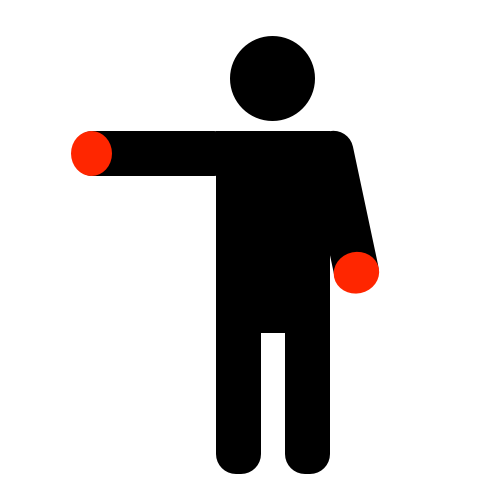
\includegraphics[height=120px]{figs/technical_challenges/kick-in.png}
        \caption{\color{blue}Kick-in \textlangle{}blue\textrangle{} Team}
    \end{subfigure}
    \begin{subfigure}{.33\textwidth}
        \centering
        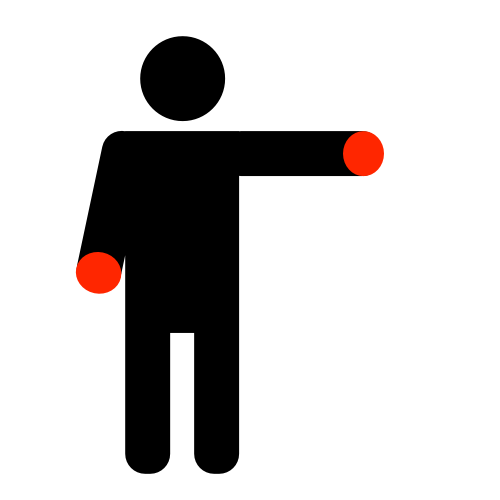
\includegraphics[height=120px]{figs/technical_challenges/kick-in-flipped.png}
        \caption{\color{red}Kick-in \textlangle{}red\textrangle{} Team}
    \end{subfigure}
    \caption{\textbf{Kick-in \textlangle{}color\textrangle{} Team.} One-handed signal. One arm, extended horizontally in the direction of the half of the field corresponding to the team that receives the Kick-in Free Kick. That is, right arm extended for the ``Blue team'', and left arm extended for the ``Red team''. The non-signal hand is flat and motionless by the side of the body.}
\end{figure*}
    
\begin{figure}[ht!]
    \centering
    \begin{subfigure}{.33\textwidth}
        \centering
        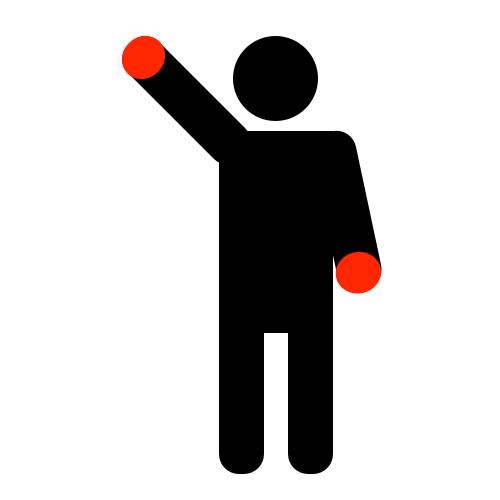
\includegraphics[height=120px]{figs/technical_challenges/goal-kick.png}
        \caption{\color{blue}Goal Kick \textlangle{}blue\textrangle{} Team}
    \end{subfigure}
    \begin{subfigure}{.33\textwidth}
        \centering
        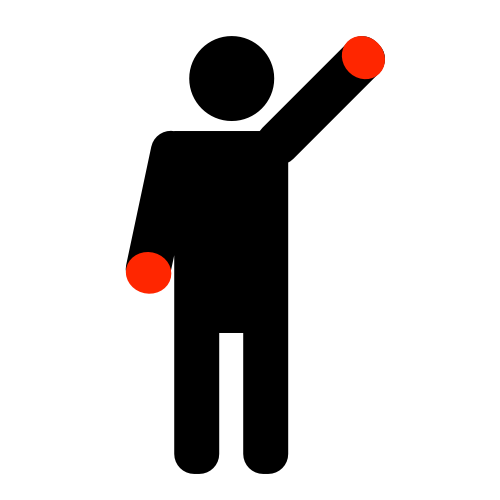
\includegraphics[height=120px]{figs/technical_challenges/goal-kick-flipped.png}
        \caption{\color{red}Goal Kick \textlangle{}red\textrangle{} Team}
    \end{subfigure}
    \caption{\textbf{Goal Kick \textlangle{}color\textrangle{} Team.} One-handed signal. One arm, extended 45-degree \emph{up} in the direction of the end of the field where the goal kick will occur. That is, right arm extended for the ``Blue team'', and left arm extended for the ``Red team''. The non-signal hand is flat and motionless by the side of the body.}
\end{figure}

\begin{figure}[ht!]
    \centering
    \begin{subfigure}{.33\textwidth}
        \centering
        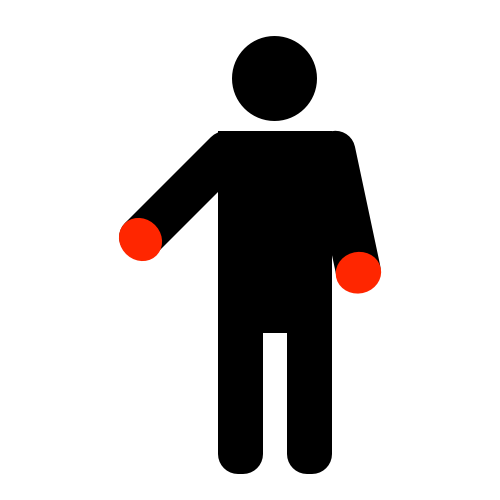
\includegraphics[height=120px]{figs/technical_challenges/corner-kick.png}
        \caption{{\color{blue}Corner Kick \textlangle{}blue\textrangle{} Team}\\ (on the half of the {\color{red} red} team)}
    \end{subfigure}
    \begin{subfigure}{.33\textwidth}
        \centering
        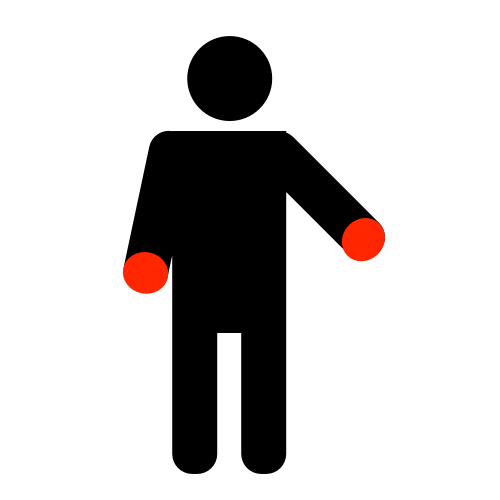
\includegraphics[height=120px]{figs/technical_challenges/corner-kick-flipped.png}
        \caption{{\color{red}Corner Kick \textlangle{}red\textrangle{} Team} (on the half of the {\color{blue} blue} team)}
    \end{subfigure}
    \caption{\textbf{Corner Kick \textlangle{}color\textrangle{} Team.} One-handed signal. One arm, extended 45-degree \emph{down} in the direction of the team executing the corner kick. That is, right arm extended for the ``Blue team'' executing the corner kick on the ``Red team's'' side, and left arm extended for the ``Red team'' executing the corner kick on the ``Blue team's'' side. The non-signal hand is flat and motionless by the side of the body.}
\end{figure}
    
\begin{figure}[ht!]
    \centering
    \begin{subfigure}{.33\textwidth}
        \centering
        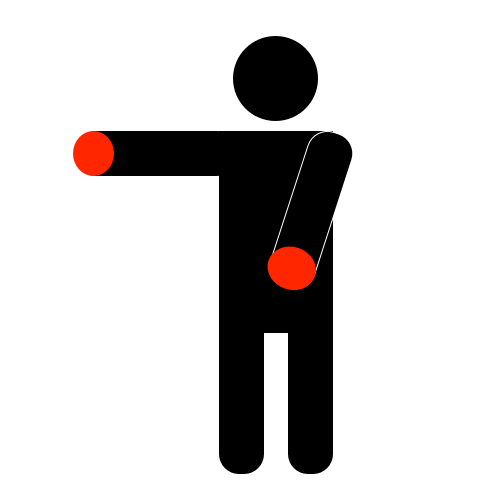
\includegraphics[height=120px]{figs/technical_challenges/goal.png}
        \caption{\color{blue}Goal \textlangle{}blue\textrangle{} Team}
    \end{subfigure}
    \begin{subfigure}{.33\textwidth}
        \centering
        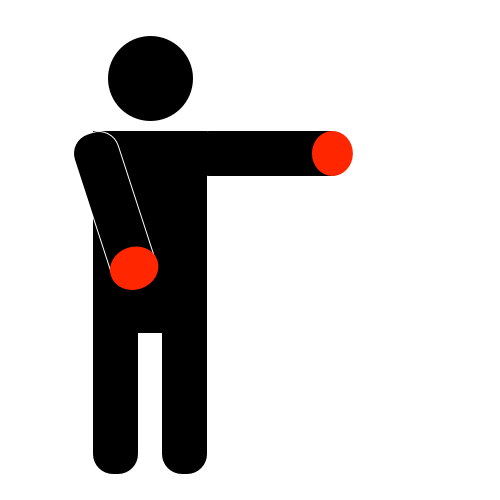
\includegraphics[height=120px]{figs/technical_challenges/goal-flipped.png}
        \caption{\color{red}Goal \textlangle{}red\textrangle{} Team}
    \end{subfigure}
    \caption{\textbf{Goal \textlangle{}color\textrangle{} Team.} Two-handed signal. One arm, extended pointing at the center circle. Other arm, extended horizontally in the direction of the half of the field corresponding to the team that scored the goal. That is, right arm extended for the ``Blue team'', and left arm extended for the ``Red team''.}
\end{figure}

\begin{figure}[ht!]
    \centering
    \begin{subfigure}{.33\textwidth}
        \centering
        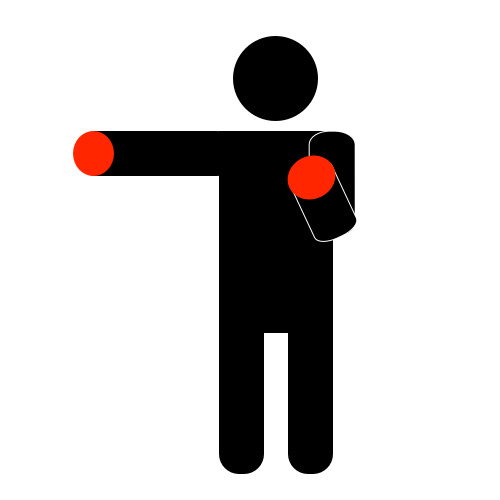
\includegraphics[height=120px]{figs/technical_challenges/pushing.png}
        \caption{{\color{blue}Pushing Free-kick \textlangle{}blue\textrangle{} Team}\\ because a {\color{red}red} robot has pushed.}
    \end{subfigure}
    \begin{subfigure}{.33\textwidth}
        \centering
        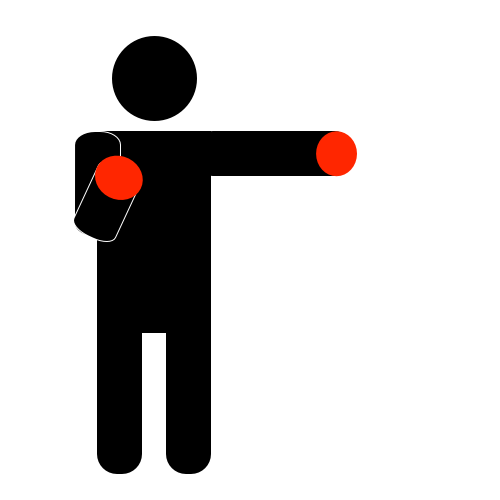
\includegraphics[height=120px]{figs/technical_challenges/pushing-flipped.png}
        \caption{{\color{red}Pushing Free-kick \textlangle{}red\textrangle{} Team}\\ because a {\color{blue}blue} robot has pushed.}
    \end{subfigure}
    \caption{\textbf{Pushing Free-kick \textlangle{}color\textrangle{} Team.} Two-handed signal. One arm, vertical with bent elbow and palm facing in the direction of the extended arm. Other arm, extended horizontally in the direction of the half of the field corresponding to the team that is \emph{executing} the Free-kick. That is, left arm extended for the ``Red team'', and right arm extended for the ``Blue team''.}
\end{figure}

\begin{figure}[ht!]
    \centering
    \begin{subfigure}{.33\textwidth}
        \centering
        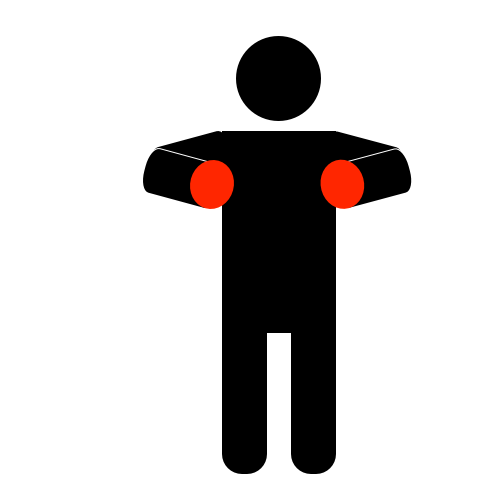
\includegraphics[height=120px]{figs/technical_challenges/full-time-start.png}
        % \caption{Inner start point of the dynamic movement}
    \end{subfigure}
    \begin{subfigure}{.33\textwidth}
        \centering
        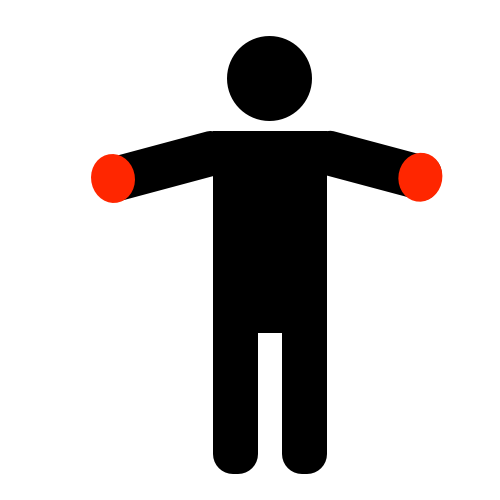
\includegraphics[height=120px]{figs/technical_challenges/full-time-end.png}
        % \caption{Outer start point of the dynamic movement}
    \end{subfigure}
    \caption{\textbf{Full-Time.} Dynamic two-handed signal. Both arms slowly move symmetrically inward and outwards on a horizontal plane, bending at the elbows.}
\end{figure}

\begin{figure}[ht!]
    \centering
    \begin{subfigure}{.33\textwidth}
        \centering
        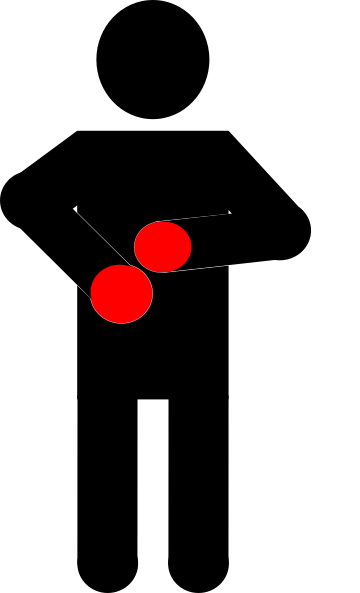
\includegraphics[height=105px]{figs/technical_challenges/substitution.png}
        \vspace*{0.5em}
        \caption{Rotation around virtual axis to indicate substitution.}
    \end{subfigure}
    \hspace*{0.5em}
    \begin{subfigure}{.6\textwidth}
        \centering
        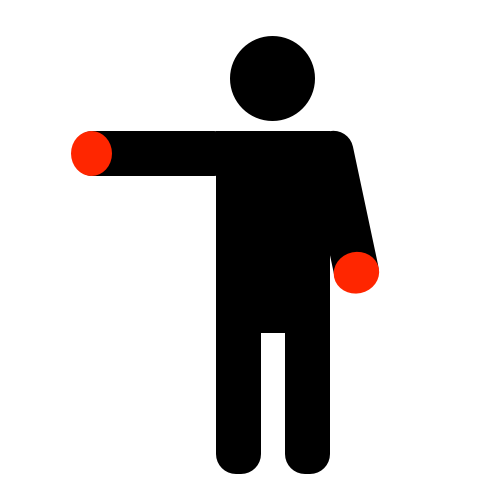
\includegraphics[height=120px]{figs/technical_challenges/kick-in.png}
        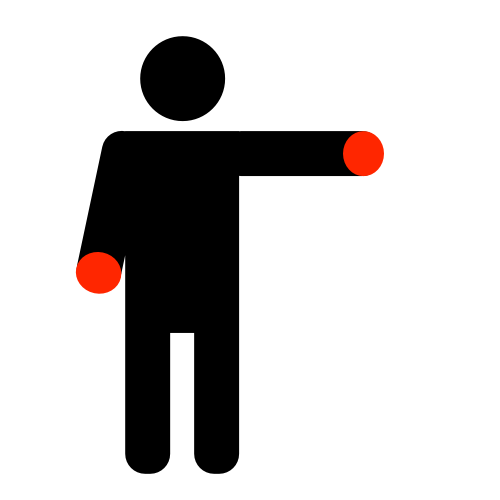
\includegraphics[height=120px]{figs/technical_challenges/kick-in-flipped.png}
        \caption{Kick-in signal to indicate the team which is substituting a player. Two possible directions.}
    \end{subfigure}
    \caption{\textbf{Substitution.} Dynamic two-handed signal. Both arms slowly rotate symmetrically around a virtual horizontal axis parallel to the touchline. After three rotations the referee indicates the team which is substituting a player with the kick-in signal.}
\end{figure}

\clearpage
\newpage

\subsection{Challenge Evaluation}

A team scores 1 point for every direction (team blue, team red or none) and 1 point for every hand-signal (ignoring the direction) correctly identified.
The time it takes a team to report a hand-signal (relative to the when signaling started, as calculated by the GameController) is recorded.
If a team does not report any hand-signal within the time limit, the time for the hand-signal is \qty{15}{\second}.
For incorrect reports, the time is how long that incorrect report took.

As the head referee only whistles in three different match situations (kick-off, goal, end of half), the signals are categorized accordingly. The average points and time per category will be calculated. The average points $\bar{P}_{\mathrm{XXX}}$ are summed with weighting factors as well as the average time $\bar{T}_{\mathrm{XXX}}$:

\begin{equation*}
    \Sigma_\mathrm{Points} = \bar{\mathrm{P}}_{\mathrm{kick\_off}} + 3 \times \bar{\mathrm{P}}_{\mathrm{goal}} + 2 \times \bar{\mathrm{P}}_{\mathrm{end\_of\_half}}
\end{equation*}
\begin{equation*}
    \Sigma_\mathrm{Time} = 3 \times \bar{\mathrm{T}}_{\mathrm{kick\_off}} + \bar{\mathrm{T}}_{\mathrm{goal}} + 2 \times \bar{\mathrm{T}}_{\mathrm{end\_of\_half}}
\end{equation*}

These two values will be determined for each match. After the preliminary matches have been finished, the minimum number of matches each team has played will be evaluated over all teams referenced as $N$. For each team the total number of points and the total time is calculated as the sum of the $N - 1$ best ranked matches according to the number of points.

Teams are ranked by their total number of points. In the case of a tie, the team with the fastest total time to identify the hand-signals is ranked higher. The team with the highest total number of points, and lowest total time (for tie-breakers), wins this in-game challenge.
